\paragraph{}This chapter presents the methodology behind the development and testing of the \ac{SLAM} tuning module developed within \ac{RUSTLE}. It begins by explaining what \ac{RUSTLE} is and how it works and then explain how the tuning module fits in with \ac{RUSTLE} and its codebase. Then, lower level details of each implemented tuning algorithm will be explained. Finally, a testing methodology will be introduced and properly explained.

\section{\acs{RUSTLE}}

\begin{figure}[h]
    \centering
    \includegraphics[page=2,width=\linewidth]{images/rustle_diagram.pdf}
    \caption{\ac{RUSTLE} software architecture}
    \label{rustle_diagram}
\end{figure}

\paragraph{}\ac{RUSTLE} is a command line application, written in Rust, which is designed to simplify the evaluation of SLAM algorithms in mobile robotics.
Its main objective is to provide a simple, streamlined and reproducible way to run and compare SLAM algorithms. It tracks not only trajectory accuracy (APE or RPE), but also runtime, CPU load and memory usage, offering a complete assessment of the algorithm's performance.

\paragraph{}At its core, RUSTLE takes three main inputs: a dataset with raw sensor data in rosbag\footnote{\url{https://wiki.ros.org/rosbag}} format, the SLAM algorithm's parameters in yaml format, and the algorithms themselves as Docker\footnote{Docker is a containerization platform that packages an application and its dependencies into lightweight, portable containers, ensuring consistent behavior across different systems. It enables reproducible environments and simplifies deployment by isolating software from the host system configuration.} images. The reason for using Docker is for reliably reproducing the algorithms across many different platforms and environments.
During execution, the estimated pose data is streamed into the database, which, after conclusion, is used to calculate trajectory errors such as the \ac{APE} and the \ac{RPE}, using EVO~\cite{grupp2017evo} (Figure \ref{rustle_diagram}).

\paragraph{}Algorithm executions are run as tests. Each test's configuration is described in an YAML file, which contains: its name, number of workers, number of iterations, list of algorithms, dataset on which to execute these algorithms and the test type. Additionally, some additional fields might be required, depending on the type of test to be executed.

%% Explicar os vários tipos de testes
\paragraph{}Tests can be of a few different types, namely:
\begin{itemize}
	\item Simple - The rosbag file simply plays from begining to end at normal speed
	\item Speed - Portions of the dataset are run at different speeds
	\item Cut - Only specified portions of the dataset are run
	\item Drop - Simulates sensor dropout, by reducing sensor message rate over a specified section of the dataset
\end{itemize}

\paragraph{}Every tuning configuration on \ac{RUSTLE} will be run as a simple test, with the caveat that the user can choose the portion of the dataset to run. This is to facilitate development and testing. %When used in production, the user should set both the start and duration of the dataset to 0, meaning, the whole dataset will be run.

%\paragraph{}The way the user interacts with the application is via a Command Line Interface(CLI), by issuing commands, such as "\textbf{cargo run -p rustle-cli algo add -f examples/algorithms.yaml}" to add one or more algorithms to the database using a settings file, or "\textbf{cargo run -p rustle-cli dataset add -f examples/datasets.yaml}", to add one or more datasets to the database. Similarly, the tuning module will require similarly structured commands, more specifically "\textbf{cargo run -p rustle-cli tune add -f examples/tune\_test.yaml}" to add a new tuning execution, whose settings are specified by in the YAML configuration file, and "\textbf{cargo run -p rustle-cli tune run grid\_test}" to run the specified tuning test.

\section{Feature Implementation}

\paragraph{}In the previous chapter, several tuning approaches were discussed, but only Grid Search, Random Search and Simulated Annealing were implemented. These three specific methods were chosen as a way to balance time efficiency and fine tuned exploration. Grid Search is an exhaustive baseline method. The user chooses how fine grained the parameter space is and the algorithm explores it sequentially. Random Search is a natural improvement over Grid Search, allowing for a more time efficient \textbf{random} exploration of the parameter space. Finally, Simulated Annealing is a meta-heuristic that introduces a temperature-controlled acceptance mechanism. %Better solutions are always accepted, but worse solutions are also occasionally accepted, according to a probability some function. This allows for a more efficient and informed exploration of the parameter space.

%\paragraph{}In addition to the optimization algorithms, it will also be necessary to write code for exporting results of a tuning test, for later result extraction, processing and discussion, as well as code for parsing a YAML settings file, with all necessary information to run the optimization experiment. Finally, some python scripts will be developed to plot the results of the tuning experiments, which will be presented in the next chapter of this dissertation. Below is a high-level diagram of the features I intend to implement.

\paragraph{}Figure \ref{low_level_tune_module} displays a low-level diagram of the tuning module developed in Rust and which was integrated into the \ac{RUSTLE} codebase. The user first creates a YAML configuration file with the \ac{SLAM} algorithm to be optimized, the dataset on which to optimize the algorithm, the \ac{SLAM} parameters to tune, any halting conditions, and other relevant data (algorithm dependent). Then, when running the optimization test, the code will keep track of the best configuration found so far, as well as some relevant data, such as parameter and \ac{RPE} values at each iteration of the algorithm, and export that data. The best configuration is written to a YAML file and the \textbf{per iteration} data is written to a csv file, for later processing.

% diagrama alto-nível das features(feito em powerpoint)
\begin{figure}[h]
    \centering
    \includegraphics[page=3,width=0.8\linewidth]{images/rustle_diagram.pdf}
    \caption{Low-level diagram of hyperparameter tuning module.}
    \label{low_level_tune_module}
\end{figure}



\newpage

\subsection{Grid Search}

\paragraph{}The Grid Search implementation considers the parameter space as a multi dimensional tensor, where each dimension corresponds to a different parameter, and has a differing number of possible values. In each iteration, to obtain the current values of the parameters

\begin{figure}[h]
\centering
\begin{algorithm}[H]
\caption{Grid Search}
\begin{algorithmic}[1]
\For{$t = 1, 2, ..., n$}
	\State Obtain the corresponding values of the parameters from the index of the configuration
	\State Evaluate the configuration and extract metrics
	\State If halting conditions are met(time limit or number of configurations), stop the algorithm's execution
\EndFor
\end{algorithmic}
\end{algorithm}
\caption{Grid Search procedure}
\label{bo_algo}
\end{figure}

\paragraph{}The halting conditions can be customized via a YAML configuration file. Similarly, the parameter space can be designed in the following way:

\begin{equation}
	parameter\_name: [first\_value,  step\_size,  number\_of\_values]
	\label{parameter_space_equation}
\end{equation}

\paragraph{}Additionally, the code looks for and catches most common errors, such as the user passing a String for a parameter that is supposed to be an integer.

\subsection{Random Search}

\paragraph{}The Random Search Implementation is similar to Grid Search, except that the index of the configuration to be evaluated is randomly generated, and no configuration is evaluated twice, by way of checking a list of previously evaluated configurations.

\begin{figure}[h]
\centering
\begin{algorithm}[H]
\caption{Random Search}
\begin{algorithmic}[1]
\For{$t = 1, 2, ..., n$}
	\State Generate a random number between in the interval [0, n], and check if the number is on the previously generated numbers list. If it is, keep generating numbers until it is not.
	\State Add the number to the previously generated numbers list.
	\State Obtain the parameter's current values and update the \ac{SLAM} configuration
	\State Evaluate the configuration and extract metrics
	\If{(elapsed\_time > time\_limit) or (evaluated\_configs > max\_iterations)}
		   		suspend algorithm execution
	\EndIf
\EndFor
\end{algorithmic}
\end{algorithm}
\caption{Random Search procedure}
\label{bo_algo}
\end{figure}

\paragraph{}As in Grid Search, in Random Search, both the parameter space and the halting conditions can be specified in a YAML configuration file.

\subsection{Simulated Annealing}

\paragraph{}The Simulated Annealing algorithm implementation is identical to the one provided by Stefan Kroboth~\cite{argmin_ref}. It is open source and written in Rust, and only small modifications had to be made for a seamless integration with \ac{SLAM} tuning.

\paragraph{}Perturbation functions are responsible for generating a new candidate solution. For simplicity's sake, only a Gaussian perturbation function was implemented for continuous parameters and a Uniform perturbation function for discrete parameters.

\paragraph{}For continuous parameters, the used Gaussian perturbation function samples a number from a  Gaussian distribution and adds the sampled value to the current value of the parameter (see Equations \ref{pert_float1} and \ref{pert_float2}). Both the mean and standard deviation of this normal distribution are unique to each parameter and can be specified in a YAML configuration file.

\paragraph{}For any continuous parameter $v$:
\begin{equation}
	v_{i + 1} = v_{i} + \Delta_v
	\label{pert_float1},
\end{equation}

\begin{equation}
	\Delta_{v} \sim \mathcal{N}(\mu, \sigma^2)
	\label{pert_float2}.
\end{equation}

\paragraph{}For non binary discrete parameters, a maximum step size is specified for each parameter, and a random number is generated within a range whose bounds are specified by the maximum step size and the temperature (see Equation~\ref{delta_int}), so it scales up and down with temperature variations.

\paragraph{}For any non binary discrete parameter $k$:
\begin{equation}
	k_{i + 1} = k_i + \Delta_k
	\label{int_param_perturbation},
\end{equation}

\begin{equation}
	\Delta_{k} \in [-T_i * max\_step, T_i * max\_step]
	\label{delta_int}.
\end{equation}

\paragraph{}Another important aspect of Simulated Annealing is the reannealing process. During the execution of the algorithm, it is sometimes necessary to reanneal, that is, to reset the temperature to a previous, higher level, to allow the algorithm to escape (or at least attempt to escape) from local minima. With that in mind, reannealing occurs under three circumstances. The algorithm automatically resets its temperature after a fixed number of iterations; it also does so when no neighboring solution is accepted for a specified stretch of consecutive iterations, and when, after a series of consecutive iterations, no candidate improves upon the current incumbent solution.

%With that in mind, 3 parameters are necessary:

%\begin{itemize}
	%\item reanneal\_fixed - the algorithm resets the temperature no matter what after this many iterations  
	%\item reanneal\_accepted - the algorithm resets the temperature if no neighbor solution is accepted after this many \textbf{consecutive} iterations
	%\item reanneal\_best - the algorithm resets the temperature if no solution better than the incumbent is found after this many \textbf{consecutive} iterations
%\end{itemize}

\paragraph{}As for halting conditions, similarly to reannealing, the algorithm stops its execution if one of three conditions are satisfied. The algorithms stops its execution after a specified maximum number of iterations; it also does so if no neighboring solution is accepted for a specified stretch of consecutive iterations or when, after a series of consecutive iterations, no candidate improves upon the current incumbent solution.

%2 parameters are specified:

%\begin{itemize}
	%\item stop\_accepted - The algorithm stops its execution if this no neighbor solution is accepted for these many \textbf{consecutive} iterations
	%\item stop\_best - the algorithm stops its execution if no solution better than the incumbent is found after these many \textbf{consecutive} iterations
%\end{itemize}

%\paragraph{}What i will be doing: explain the features i will be developing, where my code inserts itself inside of RUSTLE, which optimization strategies will be implemented and why, what tests i will do to test the code and to extract results.

\section{Testing}

\subsection{Algorithms}

%\paragraph{}In this subsection, I explain both the \ac{SLAM} methods I chose to optimize and the hyperparameters I chose to optimize and why.
\paragraph{}This subsection discusses the \ac{SLAM} methods used to test the implemented tuning algorithms and why they were chosen.

\paragraph{}While almost any \ac{SLAM} method could be used to demonstrate the results of the implementations of the tuning algorithms mentioned previously, both Faster-LIO and Fast-LIVO2 were chosen for specific reasons. Both Faster-LIO and Fast-LIVO2 are state of the art solutions and are used extensively in the recent literature~\cite{fasterlio_article1, fasterlio_article2, fasterlio_survey, fastlivo2_article1, fastlivo2_article2}.

\subsubsection{Faster-LIO}

\paragraph{}Faster-LIO was selected as the \ac{LiDAR}–inertial \ac{SLAM} system in this dissertation due to its demonstrated real-time performance and competitive accuracy in recent literature~\cite{fasterlio_article1, fasterlio_comparison}. The method employs a tightly coupled LiDAR–IMU formulation based on an iterated Kalman filter~\cite{fasterlio_article1}, enabling efficient local state estimation without relying on loop closure or global optimization. This property makes Faster-LIO well suited for analyzing the influence of hyperparameter choices on odometry accuracy under controlled conditions. In addition, the algorithm exposes a compact yet meaningful set of tunable parameters, which is appropriate for systematic hyperparameter optimization.

\subsubsection{Fast-LIVO2}

\paragraph{}Fast-LIVO2 was chosen as a complementary SLAM system to extend the analysis to a multi-modal LiDAR–visual–inertial system. By integrating visual information into the same tightly coupled estimation framework~\cite{fastlivo2_article1} (see Figure \ref{fast-livo2 system overview}), Fast-LIVO2 allows for a controlled investigation of how additional sensing modalities affect both system performance and hyperparameter sensitivity.

% diagrama alto-nível das features(feito em powerpoint)
\begin{figure}[h]
    \centering
    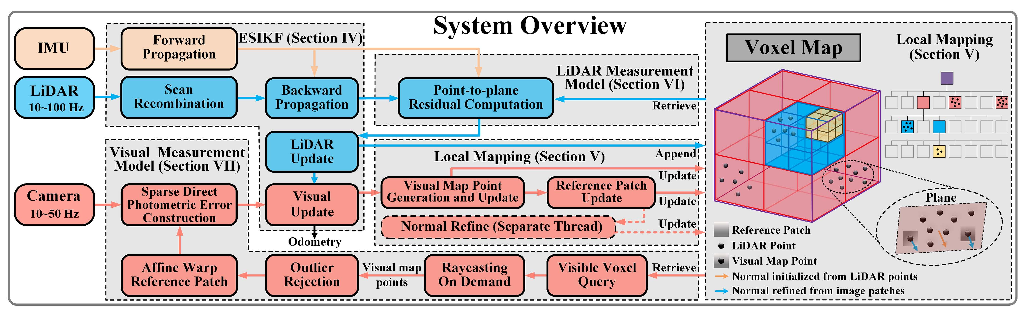
\includegraphics[page=1,width=1\linewidth]{images/fast-livo2.pdf}
    \caption{Fast-LIVO2 system overview~\cite{fastlivo2_article1}}
    \label{fast-livo2 system overview}
\end{figure}

\subsection{Metrics}

\paragraph{}During the development, as well as during testing stages, only the \ac{RPE} was considered for the calculation of the fitness function. The reason is fairly simple: both Faster-LIO and Fast-LIVO2 do not have loop closure mechanisms; as a result, the \ac{APE} is inherently high. Consequently, optimizing directly for the \ac{APE} would neither reduce nor eliminate this error, as trajectory drift would continue to accumulate, albeit at a slower rate. Despite this, the user can attribute weights to both the \ac{APE} and \ac{RPE} using a YAML configuration file. In addition, the implementation supports, with a few small modifications, to take into account other metrics (CPU load, memory usage, etc).

\subsection{Dataset}

\paragraph{}During code development, and also during testing and result extraction, the BotanicGarden dataset~\cite{Liu_2024}, specifically the 1006\_03 sequence was used. This dataset presents a challenging, semi-structured, environment (see Figure \ref{botanic garden bird view}) with diverse sensor modalities, including a DALSA M1930 stereo camera, a DALSA C1930 stereo camera, a Velodyne VLP16 \ac{LiDAR}, a Livox Avia \ac{LiDAR}, and an Xsens Mti-680G \ac{IMU}. All sensors are hardware-synchronized, ensuring time-aligned measurements suitable for sensor fusion. It also provides a robust ground truth, generated using a static terrestrial laser scanner to acquire high-density, high-resolution point clouds. These point clouds were subsequently aligned to produce ground truth trajectories with an accuracy of approximately 1 cm.

\begin{figure}[h]
    \centering
    \includegraphics[page=1,width=0.75\linewidth]{images/botanic garden.pdf}
    \caption{A bird view of the 3D survey map of BotanicGarden~\cite{liu2024botanicgarden}}
    \label{botanic garden bird view}
\end{figure}

\subsection{Tuning Strategy}

\paragraph{}For both Faster-LIO and Fast-LIVO2, a simple tuning strategy as devised., which aims to demonstrate the advantage of hyperparameter optimization in comparison to default parameters, as well as to compare the effectiveness of each implemented tuning algorithm. As for each tuned parameters in both Faster-LIO and Fast-LIVO2, the lower and upper bounds were chosen based on previous experience with these methods, mainly during the development and debugging of the tuning algorithms. Given the parameter bounds, appropriate parameter spaces were designed for Grid/Random Search, aimed at a runtime of 5 hours, and then both tuning algorithms were executed. As for Simulated Annealing, it is marginally more complex. As explained before, perturbation functions have their own settings parameters, the delta\_max for discrete parameters and the mean and standard deviation of the gaussian distribution for non discrete parameters. That being said, several runs of Simulated Annealing were needed to adjust these parameters before they allowed for a proper exploration of the previously defined parameter space (within the defined bounds).

%\paragraph{}The second test is simpler, and aims to validate the first test's results, by running both default parameters and optimized parameter configurations on another dataset. The goal is to test how generalizable an optimized configuration is to other datasets. All tuning efforts were done on the 1006\_03 sequence of the BotanicGarden dataset, while the validation was done on the 1018\_13 sequence of the BotanicGarden dataset.

\subsection{Machine}

\paragraph{}All tests were conducted on a machine with the specifications listed in Table \ref{test-machine-specs}.

\begin{table}[h]
\centering
\begin{tabular}{|c|c|}
\hline
CPU    & AMD Ryzen 7 2700x 3.7GHz    \\ \hline
GPU    & Nvidia GeForce GTX 1060 6GB \\ \hline
Memory & 16GB                        \\ \hline
Disk   & 1TB SSD + 1TB HDD           \\ \hline
OS     & Ubuntu 20.04.6 LTS          \\ \hline
Kernel & 5.15.0-139-generic          \\ \hline
\end{tabular}
\caption{Test machine specifications}
\label{test-machine-specs}
\end{table}